\chapter{Сложный атом}

\section{Вариационный принцип вычисления энергии основного состояния}

Пусть для системы с гамильтонианом $\op{H}$ задача решена, то есть найдены значения энергии $E_n$ и волновые функции $\Psi_n$, такие что:
$$
\op{H}\Psi_n = E_n \Psi_n,~~ n = 0,1,2...
$$
Волновые функции $\Psi_n$ ортонормированы,
$$
\bk{\Psi_n}{\Psi_m} = \delta_{nm}
$$
и образуют полный базис.\\
$N \geqslant 2$

Рассмотрим произвольную волновую функцию $\Phi$, нормированную на единицу:
$$
\bk{\Phi}{\Phi} = 1
$$
её разложение по базису $\Psi_n$ имеет вид:
$$
\Phi = \sum_n a_n \Psi_n
$$
В силу условий нормировки для коэффициентов $a_n$ имеем:
$$
\sum_n \abs{a_n}^2 = 1
$$
Оценим среднюю энергию $\avg{E}$ системы в состоянии, описываемой произвольной волновой функцией $\Phi$:
\begin{equation}
\label{eq:18_1_1}
\avg{E} \equiv \bfk{\Phi}{\op{H}}{\Phi} \equiv \mathcal{E}[\Phi] = \sum_n \sum_m \bfk{a_n \Psi_n}{\op{H}}{a_m \Psi_m} = \\ = \sum_n \sum_m a_n^* a_m E_m \delta_{nm} = \sum_n \abs{a_n}^2 E_n
\end{equation}
В \eqref{eq:18_1_1} $E_1, E_2, ... \to E_0$,~ $E_n \geqslant E_0$ при $\forall n$

\begin{equation}
\label{eq:18_1_2}
\boxed{\mathcal{E}[\Phi] \geqslant E_0 \sum_n \abs{a_n}^2 = E_0}
\end{equation}
Средние значения, вычисленные с пробными функциями $\Phi$, являются оценками сверху для точной энергии основного состояния (рис. \eqref{fig:18_1}).

\begin{figure}[h!]
\centering
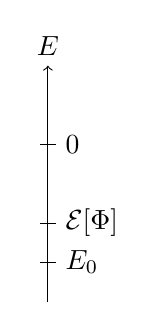
\begin{tikzpicture}[domain=-1.5:1.5]
  \draw[->] (0,-2) -- (0,1) node[above] {$E$};
  \draw[-] (-0.1,0) -- (0.1, 0) node[right] {$0$};
  \draw[-] (-0.1,-1) -- (0.1,-1) node[right] {$\mathcal{E}[\Phi]$};
  \draw[-] (-0.1,-1.5) -- (0.1, -1.5) node[right] {$E_0$};
\end{tikzpicture}
\caption{Соотношение между энергиями.} \label{fig:18_1}
\end{figure}


Если $\Phi = \Psi_0$, то $\mathcal{E}[\Psi_0] = E_0$. 

Другая формулировка:
\begin{equation}
\label{eq:18_1_3}
\mathcal{E}[\Phi] \to \min
\end{equation}

\underbar{Метод вариационного исчисления}:
\begin{equation}
\label{eq:18_1_4}
\delta \mathcal{E} = 0 ~~~ \forall \delta\Phi:~ \bk{\Phi}{\Phi} = 1
\end{equation}

\begin{enumerate}
\item Выбирается пробная функция $\Phi = \Phi(q, \alpha_1, \alpha_2 ... )$, зависящая от полного набора координат $q$ и вариационных параметров $\alpha_i$;
\item Вычисляется средняя энергия в состоянии, описываемом данной функцией:
$$
\bfk{\Phi}{\op{H}}{\Phi} = \mathcal{E}(\alpha_1, \alpha_2 ...)
$$
\item Минимизируем $E$ по вариационным параметрам:
$$
\pd{\mathcal{E}}{\alpha_1} = 0,~~ \pd{\mathcal{E}}{\alpha_2} = 0, ... 
$$
Находим соответствующие $\alpha_i^0$.
\end{enumerate}
После этого можно утверждать, что функция $\Phi(q, \alpha_1^0, \alpha_2^0, \alpha_2^0 ...)$ есть наилучшее приближение к $\Psi_0(q)$ в выбранном классе функций. (см. задачи 2 и 3 из II задания)

В \eqref{eq:17_2_1}: $\nu = 1s$, $S = 0 \uparrow \downarrow$
\begin{equation}
\label{eq:18_1_5}
\Phi_{g.s}^{S}(\vr_1, \vr_2) = \phi_{1s}(\vr_1)\phi_{1s}(\vr_2) = \frac{1}{\pi} \brc{\frac{Z}{a}}^3 e^{-\frac{Z(r_1 + r_2)}{a}}
\end{equation}
--- отсутствуют вариционные параметры.

Эффективный заряд $\tilde{Z} < Z = 2$

\begin{equation}
\label{eq:18_1_6}
\Phi_{g.s}(\vr_1, \vr_2) = C e^{-\frac{\tilde{Z}(r_1 + r_2)}{a}}
\end{equation}
$$
\bfk{\Phi_{g.s}^{S}}{\op{H}}{\Phi_{g.s}^{S}} = \mathcal{E}(\tilde{Z})
$$
$$
\pd{\mathcal{E}}{\tilde{Z}} = 0 ~~\to~~ \tilde{Z} = Z - \frac{5}{16}
$$
--- задача 3а из второго задания. В задаче 3б два вариационных параметра: $\alpha$ и $\beta$.

\section{Метод Хартри-Фока. Приближения центрального поля. Электронные конфигурации}
$N$ электронов, заряд $-Ze~~ (e<0)$
\begin{equation}
\label{eq:18_2_1}
\op{H} = \sum_{i=1}^{N} \brc{\frac{\op{\vp_i}^2}{2m} - \frac{Ze^2}{r_i}} + \sum_{i<j} \frac{e^2}{\abs{\vr_i - \vr_j}}
\end{equation}

Эффективное среднее поле --- метод Хартри-Фока (1928-1930).

\begin{enumerate}
\item \begin{equation}
\label{eq:18_2_2}
\mathcal{E}\brs{\{\psi_{\{n_j\}}(\xi_i)\}} = \bfk{\Uppsi^{HF}}{\op{H}}{\Uppsi^{HF}}
\end{equation}

\item $\psi_{\{n_j\}}(\xi_i)$ - спин-орбиталь,  $\Uppsi^{HF}(\xi_1, \xi_2, ... \xi_N) = Slater~determinant$ (см. \eqref{eq:16_2_2})

\item 
$$
\mathcal{E}\brs{\{\psi_{\{n_j\}}(\xi_i)\}} = \min~ \forall \delta\psi_{\{n_j\}}(\xi_i)
$$
\end{enumerate}

Система из $N$ уравнений $\to$ уравнения Хартри-Фока. Каждое из них описывает движение выделенного $i$-го электрона в некотором эффективном \underbar{среднем поле} $U_{cc}(\vr_i)$, созданным ядром и остальными электронами атома. 

$U_{cc}(\vr_i)$ --- центральное, \underbar{самосогласованное} поле (ССП, SCF).

Из \eqref{eq:18_2_1}:
$$
\op{H} = \underbrace{\sum_{i=1}^{N} \brc{\frac{\op{\vp_i}^2}{2m} + U_{cc}(\vr_i)}}_{\op{H}^{(0)}} + \op{V}
$$
где $\op{H}^{(0)}$ --- центральная, а $\op{V}$ --- нецентральная части гамильтониана:
$$
\op{V} = \sum_{i<j} \frac{e^2}{\abs{\vr_i - \vr_j}} + \sum_{i=1}^N \brc{-\frac{Ze^2}{r_i} - U_{cc}(\vr_i)}
$$
Пусть поле центрально-симметрично: $U_{cc}(\vr_i) = U_{cc}(r_i)$
$$
U_{cc}(r_i) =
\begin{cases}
-\frac{Ze^2}{r_i},& r_i \to 0\\
-\frac{(Z-(N-1))e^2}{r_i},& r_i \to \infty\\
\end{cases}
$$

В сложных атомах энергия зависит от $n$ и $l$ ($E_{nl}$), то есть вырождение по $l$ снимается.
$$
\psi_{\{n_j\}}(\xi_i) = R_{n_j l_j}(r_i) Y_{l_j m_j}(\theta_i, \phi_i) \chi_{\frac{1}{2}} \lambda_j(\sigma_i)
$$


\begin{defn}
Совокупность состояний с заданными $n$ и $l$ называется \underline{электрон-} \underline{ной} \underline{оболочкой} атома.
\end{defn}

Таких состояний $2(2l + 1)$.

\begin{defn}
Электроны, находящиеся в состояниях с одинаковыми $n$ и $l$, называются \underline{эквивалентными}.
\end{defn}

Например, в основном состоянии $He$ его электронная конфигурация  $1s^2$, в первом возбужденном -- $1s^12s^1$.

\begin{defn}
Распределение электронов по электронным оболочкам называется электронной конфигурацией. 
\end{defn}

\begin{gather*}
M_L = \sum_{i = 1}^{2(2l+1)} m_i = 2 \sum_{i=-l}^l m_i = 0 \\ 
M_S = \sum_{i = 1}^{2(2l+1)} m_{si} \\
\op{\vec{L}} = \sum_{i = 1}^{N} \op{\vec{l}}_i \\
\end{gather*}
\begin{equation}
\label{eq:18_2_3}
\op{\vec{S}} = \sum_{i = 1}^{N} \op{\vec{s}}_i
\end{equation}
\section{Интегральное движение в сложных атомах. Термы. Правила Хунда}

\begin{excr}
Доказать, что $\op{\vec{L}}$ и $\op{\vec{S}}$ коммутируют с $\op{H}$ \eqref{eq:18_2_1}.
\end{excr}

Для операторов $\op{H}$, $\op{\vec{L}}^2$, $\op{L_z}$, $\op{\vec{S}}^2$, $\op{S_z}$ собственными векторами будут $\ket{L M_L S M_S}$.

Энергия задается выражением: 
$$
E = E(S, L) = \bfk{L M_L S M_S}{\op{H}}{L M_L S M_S}
$$ 

Уровни энергии сложного атома называются \underline{термами}.

Термы обозначаются: $\boxed{^{2s+1}L}$.

$2s+1$ - мультиплетность.

Кратность вырождения терма равна $(2s+1)(2l+1)$.

Различные значения орбитального момента обозначаются буквами:
$$ 
\begin{matrix}
L= & 0 & 1 & 2& ...\\
      & s & p & d & ... 
\end{matrix}
$$

Полный момент задается формулой:
\begin{equation}
\label{eq:18_3_1}
\op{\vec{J}} = \op{\vec{L}} + \op{\vec{S}}
\end{equation}

Из \eqref{eq:15_2_4}:
$$
J = \abs{L-S}, \abs{L-S} + 1, ..., L+S
$$

Если мы хотим учесть спин-орбитальное взаимодействие, то правильной системой собственных векторов будет $\{ \ket{J M_J L S}\}$, общая для операторов $\op{H}$, $\op{\vec{J}}^2$, $\op{J_z}$, $\op{\vec{L}}^2$, $\op{\vec{S}}^2$
\begin{gather*}
\op{H}^{SO} = \op{H} \left |_{\eqref{eq:18_2_1}} \right . + \op{V}^{SO},
\end{gather*}

где $\op{V}^{SO} = A(\vec{L}, \vec{S})$.

\begin{excr}
Доказать, что $[\op{V}^{SO}, \op{L_z}] \not = 0$ и $[\op{V}^{SO}, \op{S_z}] \not = 0$.
\end{excr}

Для проекции полного момента верно:
$$
\op{J}_z = \op{L}_z + \op{S}_z
$$

Для такой системы собственных векторов терм записывается: $\boxed{^{2s+1}L_J}$. 

При каких $J$, $L$, $S$ энергия достигает минимума?

Ответ дают \underline{правила Хунда} (1925):

\begin{enumerate}
\item Для заданной электронной конфигурации наименьшей энергией обладает терм с наибольшим возможным значением $S$ и наибольшим (возможным при этом $S$) значением $L$.
\item Минимальной энергией обладает терм с $J = \abs{L-S}$, если оболочка заполнена менее, чем наполовину, и с $J = L + S$ в противном случае.
\end{enumerate}

\section{$LS$-связь. Тонкая структура уровней. Правило интервалов Ланде}

\eqref{eq:18_2_3} - \eqref{eq:18_3_1} -- $LS$-связь (связь Рассела-Саундреса).

Термы: $^{2s+1}L_J$.

Спин-орбитальное взаимодействие можно рассматривать, как возмущение:

\begin{equation}
\label{eq:18_4_1}
\abs{V_{SO}} \ll \Delta E_T,
\end{equation}

 где $\Delta E_T$ - разность энергий между соседними термами.
 
Для тяжелых элементов существенны релятивистские эффекты:
$$
\frac{v_{\text{s электрона}}}{c} \sim \alpha Z = \frac{Z}{137}
$$

Эти эффекты становятся существенны около никеля ($Z = 28$).

Вычислим интервалы тонкой структуры:

$$
\op{V}_{SO} = A(\op{\vec{L}}, \op{\vec{S}})
$$

Кратность вырождения $(2s + 1)(2l+1)$. 

Рассмотрим вырождение по $J$. Если $L > S$, то уровней $2S+1$, а если $S> L$, то уровней $2L+1$.

Из \eqref{eq:18_3_1}:
$$
\op{\vec{J}}^2 = \op{\vec{L}}^2 + \op{\vec{S}}^2 + 2\op{\vec{L}}\op{\vec{S}}
$$

Подставим это выражение в $\op{V}_{SO}$.

\begin{equation}
\label{eq:18_4_2}
\op{V}_{SO} = A\frac{\op{\vec{J}}^2 - \op{\vec{L}}^2 - \op{\vec{S}}^2}{2}
\end{equation}

Найдем поправку к энергии, обусловленную спин-орбитальным взаимодействием:
$$
\Delta E_J = \bfk{J M_J L S}{\op{V}_{SO}}{J M_J L S} = A \frac{J(J+1) - L(L+1) - S(S+1)}{2}
$$

Это выражение не зависит от $M_J$, т.е. вырождение снимается не полностью. Каждый такой уровень является $(2J+1)$ - кратно-вырожденным.

Найдем расстояние между соседними по $J$ уровнями:

\begin{equation}
\label{eq:18_4_3}
\Delta E_{J,L,S} - \Delta E_{J-1, L, S} = \frac{A}{2}\brcr{J(J+1) - J(J-1)} = AJ
\end{equation}

- правило интервалов Ланде (1923).

Компонентами тонкой структуры называются термы расщепленного состояния.

\section{Гамильтониан сложного атома в магнитном поле}

Запишем выражение для векторного потенциала в виде:

$$
\vA(\vr) = \frac{1}{2}[\vec{\Hvec} \times \vr],
$$

где $\Div \vA = 0$.

Из \eqref{eq:14_3_2}
\begin{equation}
\label{eq:18_5_1}
\op{H}(i) = \frac{1}{2m}\brc{\op{\vp}_i - \frac{e}{c}\vA_i}^2 - \frac{e\hbar}{mc}\brc{\op{\vec{s}}_i \cdot \Hvec} + U(\vr_i),
\end{equation}

где $\vA_i = \vA(\vr_i)$, $\mu_B = -\frac{e\hbar}{2mc}$ - магнетон Бора. Напомним, что мы считаем $e < 0$.

Электроны находятся в поле ядра, а также отталкиваются друг от друга. Этим эффектам соответсвует $U(\vr_i) = \Phi(\vr_i)$.

Раскроем скобки в \eqref{eq:18_5_1}:
\begin{gather*}
\brc{\op{\vp}_i - \frac{e}{c}\vA_i}^2 = \op{\vp}_i^2 - \frac{e}{c}\brc{\op{\vp}_i \vA_i + \vA_i \op{\vp}_i} + \frac{e^2}{c^2}\vA_i^2 
\end{gather*}

С учетом выражения:
$$
\op{\vp}_i \vA_i (\cdot) = -i\hbar \nabla_i \vA_i(\vr_i)(\cdot) + \vA_i \op{\vp}_i(\cdot)
$$

Получаем:
\begin{gather*}
\brc{\op{\vp}_i - \frac{e}{c}\vA_i}^2 = \op{\vp}_i^2 - \frac{e}{c}\brc{\op{\vp}_i \vA_i + \vA_i \op{\vp}_i} + \frac{e^2}{c^2}\vA_i^2 = \op{\vp}_i^2 - 2\frac{e}{c}\vA_i \op{\vp}_i + \frac{e^2}{c^2}\vA_i^2
\end{gather*}

Теперь преобразуем второе слагаемое:
$$
2\frac{e}{c}\vA_i \op{\vp}_i = 2\frac{e}{c} \frac{1}{2}([\Hvec \times \vr_i], \op{\vp}_i) = \frac{e}{c}([\op{\vr}_i \times \op{\vp}_i], \Hvec) =\frac{e}{c}(\hbar \op{\vec{l}}_i, \Hvec)   
$$

Окончательно получаем:
\begin{gather*}
\op{\vp}_i^2 - 2\frac{e}{c}\vA_i \op{\vp}_i + \frac{e^2}{c^2}\vA_i^2 = \op{\vp}_i^2 - \frac{e\hbar}{c}(\op{\vec{l}}_i, \Hvec) + \frac{e^2}{c^2}\vA_i^2
\end{gather*}

Подставим это выражение в гамильтониан сложного атома:
\begin{gather}
\label{eq:18_5_2}
\op{H} = \sum_{i=1}^N \op{H}(i) + \op{V}_{SO} =  \nonumber \\
= \sum_{i=1}^N \left ( {\frac{\op{\vp}_i^2}{2m} - \underbrace{\frac{e\hbar}{2mc}}_{\mu_B}(\op{\vec{l}}_i, \Hvec) + \frac{e^2}{2mc^2}\vA_i^2 - \underbrace{\frac{e\hbar}{mc}}_{2\mu_B}\brc{\op{\vec{s}}_i \cdot \Hvec}} + U(\vr_i) \right ) + \op{V}_{SO} =  \nonumber \\ 
= \op{H_0} + \op{V}_Z +\op{V}_D
\end{gather}

Рассмотрим каждое слагаемое в последней формуле.

$\op{H}_0$ - гамильтониан свободного атома.
$$
\op{H}_0 =  \sum_{i=1}^N \brc{\frac{\op{\vp}_i^2}{2m}  + U(\vr_i)} + \op{V}_{SO}
$$

$\op{V}_Z = \mu_B (\op{\vec{L}} + 2\op{\vec{S}}) \Hvec$ - оператор зеемановского взаимодействия.

Можно также записать, что $\op{V}_Z = -\op{\bm{\mu}_{\text{ат}}}\Hvec,$ где $\op{\bm{\mu_{\text{ат}}}} = -\mu_B (\op{\vec{L}} + 2\op{\vec{S}})$.

$$
\op{V}_D = \frac{e^2}{2mc^2} \sum_{i=1}^N \vA_i^2 = \frac{e^2}{8mc^2} \sum_{i=1}^N [\Hvec \times \vr_i]^2 
$$ 

- оператор диамагнитного взаимодействия.

Пусть $\Hvec = (0, 0, \mathscr{H})$. Тогда
$$
\op{V}_Z = \mu_B (\op{{L}}_z + 2\op{{S}}_z) \mathscr{H}
$$

\begin{equation}
\label{eq:18_5_3}
\op{H} = \op{H}_0 + \mu_B (\op{{L}}_z + 2\op{{S}}_z) \mathscr{H} +\frac{e^2 \mathscr{H}^2}{8mc^2} \sum_{i=1}^N [\vec{n}_z \times \vr_i]^2 
\end{equation}

Когда последним слагаемым можно пренебречь?
$$
\frac{e^2 \mathscr{H}^2}{mc^2}a^2 \ll \frac{e\hbar}{mc}\mathscr{H}
$$
$$
\mathscr{H} \ll \brc{\frac{e}{a^2}} \brc{\frac{\hbar c}{e^2}} = \mathscr{E} \alpha^{-1} = \mathscr{H} \sim 10^4 \text{Гс}
$$

Таким образом, в небольшом магнитном поле можно пренебречь последней суммой. Тогда для гамильтониана получим:

\begin{equation}
\label{eq:18_5_4}
\op{H} = \op{H}_0 + \mu_B (\op{L}_z + 2\op{S}_z)\mathscr{H} = \op{H}_0 - \op{\bm{\mu_{\text{ат}}}} \Hvec
\end{equation} 

\section{Эффекты Зеемана и Пашена-Бака}

\subsection{Слабое поле}

Рассмотрим случай слабого поля:
\begin{equation}
\label{eq:18_6_1}
\boxed{\abs{V_{\mu_{\text{ат}}\Hsc}} \ll \abs{E_J - E_{J-1}}}
\end{equation}

$$
E_J = E(L, S) + \Delta E_J 
$$

Расщепление $\Delta E_J$ обусловлено зеемановским взаимодействием $\op{V}_Z$.

При $\Hvec = 0$ кратность вырождения $2J + 1$.

Выберем базис $\{ \ket{J M_J L S}\}$.

$$
\op{\vec{J}} = \op{\vec{L}} +\op{\vec{S}} 
$$

\begin{figure}[h!]
\centering
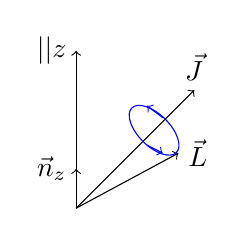
\begin{tikzpicture}[domain=-2:2]
  \draw[->] (0, 0) -- (0, 2) node[left] {$\Hvec || z$};
  \draw[->] (0, 0) -- (0, 0.5) node[left] {$\vec{n}_z$};  
  \draw[->] (0, 0) -- (1.5,1.5) node[above] {$\vec{J}$};
  \draw[->] (0, 0) -- (1.3,0.7) node[right] {$\vec{L}$};
  \draw[rotate=45, blue] (1.4, 0) ellipse (2mm and 4 mm); 
  \draw[blue, ->] (1.1, 1.15) -- (0.9,1.3) ;
  \draw[blue, ->] (0.9, 0.8 ) -- (1.1,0.7) ;

\end{tikzpicture}
\caption{К выводу эффекта Зеемана в слабом поле.} \label{fig:18_2}
\end{figure}


Из \eqref{eq:18_6_1}:
\begin{equation}
\label{eq:18_6_2}
\Omega \ll \omega_{LS},
\end{equation}

где $\Omega = \frac{\mu_B \Hsc}{\hbar}$.

Для энергий термов получим:
$$
E_{\Hsc} = E^\zr + \Delta E_{\Hsc}^\one,
$$

где 
$$
\Delta E_{\Hsc}^\one =|_{\eqref{eq:18_5_4}} \mu_B \bfk{J M_J L S}{\underbrace{\op{L}_z + 2\op{S}_z}_{\op{J}_z + \op{S}_z}}{J M_J L S} \Hsc  = \mu_B \avg{\op{J}_z + \op{S}_z} \Hsc
$$

Попробуем найти такое число $g$ (фактор Ланде), чтобы выполнялось равенство:
$$
\avg{\op{J}_z + \op{S}_z} = g\avg{\op{J}_z} \to \op{J}_z + \op{S}_z = g\op{J}_z 
$$

\begin{gather*}
\op{J}_z = \op{\vec{J}} \vec{n}_z \\
\op{S}_z = \op{\vec{S}} \vec{n}_z \\
\op{\vec{J}} \vec{n}_z \op{\vec{S}} \vec{n}_z = \brc{\op{\vec{J}} + \op{\vec{S}}}\vec{n}_z = \op{J}_z + \op{S}_z = g \op{J}_z
 = g \op{J}_z = g \op{\vec{J}} \vec{n}_z
\end{gather*}

Домножим последнее уравнение на $\op{\vec{J}}$ слева:
\begin{gather*}
\op{\vec{J}} \left |~~~ \op{\vec{J}} + \op{\vec{S}} = g\op{\vec{J}} \right . \\
g = ? \\
\avg{\op{\vec{J}}^2 + \op{\vec{J}} \op{\vec{S}}} = g \avg{\op{\vec{J}}^2} \\
\end{gather*}

Из упр.1 II задания:
$$
\avg{\op{\vec{J}} \op{\vec{S}}} = \frac{1}{2}[J(J+1) + S(S+1) - L(L + 1)]
$$

\begin{equation}
\label{eq:18_6_3}
\boxed{g = 1 + \frac{J(J+1) + S(S + 1) - L(L + 1)}{2J(J+1)}}
\end{equation}

- фактор Ланде.

\begin{equation}
\label{eq:18_6_4}
\Delta E_{\Hsc}^\one = \mu_B g \bfk{J M_J L S}{\op{J}_z}{J M_J L S} \Hsc = \boxed{\mu_B g M_J \Hsc = \Delta E_{\Hsc}^\one}
\end{equation}

$M_J = -J, -J + 1, ..., J$ - $2J+1$ значение.

\begin{figure}[h!]
\centering
\begin{tikzpicture}[domain=-5:5]
  \foreach \x in {-1.2, -0.8, -0.4, 0, 0.4, 0.8, 1.2}
    \draw[-] (1,\x) -- (2,\x) ;
  \node at (1.5, 2) {$\Hvec \neq 0$};
  \node at (-0.5, 2) {$\Hvec = 0$};
  \draw[-] (-1,0) -- (0,0) ;
  \draw[<->] (1.9, -0.8) -- (1.9,-0.4) node[right] {$\mu_B g \Hsc M_J$};
  \draw[-] (4, 1.8) -- (3.8, 1.8);
  \draw[-] (4, -1.8) -- (3.8, -1.8);
  \draw[-] (4, 1.8) -- (4, -1.8);
  \node [right] at (4, 0) {$2J+1$};
\end{tikzpicture}
\caption{Аномальный эффект Зеемана.} \label{fig:18_3}
\end{figure}

В слабом магнитном поле наблюдается аномальный эффект Зеемана (рис. \eqref{fig:18_3}) - снимается вырождение по $M_J$. Вырождение энергетического спектра атома снимается полностью.

Найдем, на каких частотах возможно излучение:

\begin{gather}
\label{eq:18_6_5}
E_1 = E_1^\zr + \mu_B g_1 M_{J1} \Hsc \nonumber \\
E_2 = E_2^\zr + \mu_B g_2 M_{J2} \Hsc \nonumber \\
\hbar \omega = E_1 - E_2 = E_1 = (E_1^\zr -E_2^\zr)  + \mu_B \Hsc (g_1 M_{J1}  - g_2 M_{J2})
\end{gather}

Однако частоты дополнительно ограничиваются правилами отбора:
$$
\boxed{\Delta L = 0, \pm 1,~~~ \Delta S = 0, ~~~\Delta J = 0, \pm 1, ~~~ \Delta M_J = 0, \pm 1 }
$$

\subsection{Сильное поле}

$$
\abs{E_J - E_{J-1}} \ll \abs{V_{\mu_{\text{ат}}\Hsc}}  \ll \Delta E_T,
$$

где $\Delta E_T$ - расстояние между соседними термами.

Ограничение сверху связано с тем, что наши выкладки верны, пока в атоме сохраняется $LS$-связь.

\begin{sloppypar}
В сильном магнитном поле наблюдается простой эффект Зеемана или эффект Пашена-Бака.
\end{sloppypar}
$\op{\vec{L}}$, $\op{\vec{S}}$ - сохраняются, поэтому необходимо пользоваться базисом $\{ \ket{L M_L S M_S}\}$.

$$
\Delta E_{\Hsc}^\one =\left |_{\eqref{eq:18_5_4}} \mu_B g \bfk{L M_L S M_S}{\op{L}_z + 2 \op{S}_z}{L M_L S M_S} \Hsc \right .
$$

\begin{equation}
\label{eq:18_6_6}
\Delta E_{\Hsc}^\one = \mu_B \Hsc(M_L + 2 M_S)
\end{equation}

$$
M_L = -L, -L + 1, ..., L
$$
$$
M_S = -S, -S + 1, ..., S
$$

В отсутствие поля, энергетический уровень $(2L+1)(2S+1)$-кратно вырожден. В магнитном поле вырождение снимается частично.
\begin{equation}
\label{eq:18_6_7}
\hbar \omega = E_1 - E_2 = E_1 = (E_1^\zr -E_2^\zr)  + \mu_B \Hsc (\Delta M_L  - 2\Delta M_S)
\end{equation}

Возможные переходы определяются правилами отбора:
$$
\boxed{\Delta L = 0, \pm 1,~~~ \Delta S = 0, ~~~\Delta M_L = 0, \pm 1, ~~~ \Delta M_S = 0}
$$
